\part{From Study 1 to Study 2: Roadmap and Design}

\chapter{The roadmap and what we did with it}
\label{r:ch:roadmap}

\section{What Study 1 left unresolved}

Study~1 (Part~II) ended with a strong benchmark-construction conclusion and a deliberately weak model-performance
conclusion. Five problems stood between them.

\begin{enumerate}[leftmargin=1.8em]
\item \textbf{One question, six tests.} ``Does crop-level splitting inflate accuracy?'' was tested once per
architecture inside a twelve-test Benjamini--Hochberg family. Every point estimate was positive, every test was
underpowered, and none survived.
\item \textbf{Availability is not use.} A 424-way probe recognised fields far above chance, but that shows the shortcut
is \emph{available}, not that classifiers route their predictions through it.
\item \textbf{Leakage confounded with diversity.} At equal crop counts a crop-level training set contains about 914
distinct fields and a field-level one about 773; P1 differs from P2 in training diversity as well as in leakage.
\item \textbf{One rescored benchmark.} Only SIPaKMeD was rescored for classification; CRIC, whose crop-level split puts a
training parent behind essentially every test cell, was not.
\item \textbf{The host.} The original classification matrix had to be repeated (Chapter~\ref{s1:ch:ch13_execution_lifecycle_failures_and_demotiv}
is the record), and runs were slower than expected for reasons only diagnosed in Study~2 (Section~\ref{r:ch:host}).
\end{enumerate}

\section{The roadmap, item by item}

The October review turned these into a phased roadmap. Table~\ref{r:tab:roadmap} records what was done with every
item, including the ones deliberately not done.

{\small
\begin{longtable}{p{0.24\textwidth}p{0.45\textwidth}p{0.22\textwidth}}
\caption{The scaling roadmap and the response to each item.}\label{r:tab:roadmap}\\
\toprule
Roadmap item & What was done & Status \\
\midrule
\endfirsthead
\toprule
Roadmap item & What was done & Status \\
\midrule
\endhead
\bottomrule
\endfoot
\multicolumn{3}{l}{\textbf{Phase 0: arXiv readiness}} \\
Fresh-clone check & Public repository cloned into a clean directory; its 45 tests pass. The public \texttt{main} branch stops at 22 August and lacks the Cx22 commits and a LICENSE file. & done; push and licence are authors' decisions \\
Text extraction of PDFs & Ligatures broke copy-paste in the drafts; \texttt{glyphtounicode} and T1 encoding added to every preamble. & done \\
Draft claims & The ISBI draft's sentence implying P3 is strictly more conservative than P2 flagged as an overreach; the draft's conclusion now says replication is in progress. & done \\
\multicolumn{3}{l}{\textbf{Phase 1: fix the statistics}} \\
Single omnibus test & One crossed mixed model, \texttt{acc \textasciitilde{} x + (1+x|architecture) + (1|seed) + (1|split)}, with the split random effect that the roadmap's formula omitted (twelve architectures share each test set). & done (H1) \\
Simulation-based power & Custom R simulation of the exact model, 1,000 simulations per design cell, from the Study~1 variance components (Chapter~\ref{r:ch:power}). & done \\
More architectures & Twelve: the six Study~1 models plus ConvNeXt-T, Swin-T, RegNetY-1.6GF, EfficientNetV2-S, MaxViT-T, and self-supervised DINOv2 ViT-S/14. & done \\
15--25 seeds & Twenty, chosen by a registered power rule. & done \\
Preregistration & \texttt{PREREGISTRATION\_STUDY2.md}, registered as Amendment~6 before any Study~2 model was trained. & done \\
Keep predictions, logits, checkpoints & Every run keeps per-crop logits, float16 final weights, and probe-split features; this is what made Amendment~8's evaluation-only arms possible. & done \\
\multicolumn{3}{l}{\textbf{Phase 2: causal arms}} \\
2C leakage vs diversity & Factorial over one common test set at matched crop and field counts. & done (H3) \\
2A fingerprint suppression & Class-conditional parent adversary behind gradient reversal, seven-level $\lambda$ sweep. & done (H5) \\
2B background transplant & Counterfactual composites with a same-parent (sibling) control. & done (H4) \\
\multicolumn{3}{l}{\textbf{Phase 3: generalisation}} \\
Other domains (fish imagery) & Gated on Phase~1 and~2 outcomes; not started. & deferred by design \\
\multicolumn{3}{l}{\textbf{Part 5: datasets}} \\
CRIC second rescore & Rescored with six architectures and ten seeds. & done (H2) \\
Keep Cx22 un-rescored & Kept; the official Cx22 split is parent-disjoint. & done \\
Cx22 literature check & Four open-access studies examined (Section~\ref{r:sec:cx22-lit}). & done \\
JUCYT ground truth & Not publicly available. & not possible \\
\multicolumn{3}{l}{\textbf{Part 6 and Part 8}} \\
Single-column neutral draft & \artifact{paper/v2}, every number generated. & done \\
Avoid scope creep & Study~2 ran only registered arms; Amendment~8 was added after Study~2's results with an explicit justification and its own Holm family. & done \\
\end{longtable}
}

\section{Phase 0 in detail}

The repository was cloned from its public remote into an empty directory, its environment created from the lock file,
and its test suite run: 45 tests passed. Three gaps were recorded in \artifact{reports/study2/phase0_arxiv_checklist.md}.
The public branch stops at 22 August 2026 and does not contain the Cx22 segmentation commits; there is no LICENSE file,
so nobody may legally reuse the toolkit; and several drafts produced PDFs whose ligatures (fi, fl) did not survive
copy-paste. The third was fixed in every preamble. The first two are decisions for the authors and remain open.

\section{The Cx22 literature check}
\label{r:sec:cx22-lit}

The Cx22 release ships an official parent-disjoint split (Multi-Train/Multi-Test). The question was whether downstream
users keep it. Of four open-access studies that train on Cx22, three use the official split. One describes image-level
five-fold cross-validation over all 1,320 generated regions, which pools regions from the same CCEDD source image across
folds. Following the project's no-naming rule for third-party work, only the aggregate is reported
(\artifact{reports/study2/cx22_literature_check.md}).

\section{Post hoc reanalysis of Study 1}

While validating the analysis code, the registered H1 model was fitted to the sixty Study~1 SIPaKMeD P1 and P2 runs. It
gives \RecPostSipEst~pp (SE \RecPostSipSE, Satterthwaite $df=\RecPostSipDf$, $p=\RecPostSipP$). The same model on the
Cx22 semantic-segmentation runs gives \RecPostCxEst\ Dice points ($p=\RecPostCxP$). Both analyses were specified after
the Study~1 data were seen; they motivated Study~2 and supplied its pilot variances, and they are not evidence for
Study~2 (\artifact{results/study2/posthoc/README.md}).

\chapter{The Study 2 preregistration}
\label{r:ch:prereg}

\begin{figure}[H]
\centering
\begin{adjustbox}{max width=\textwidth}
\begin{tikzpicture}[node distance=4mm and 4mm]
\node[box=24mm] (code) {Implement and unit-test};
\node[box=24mm, right=of code] (dry) {Synthetic dry run\\\footnotesize planted effects};
\node[box=24mm, right=of dry] (smoke) {Smoke tests\\\footnotesize crop-level only};
\node[done=24mm, right=of smoke] (reg) {Register\\\footnotesize commit + hashes};
\node[box=24mm, right=of reg] (run) {Run matrix\\\footnotesize frozen checkout};
\node[box=24mm, below=of run] (collect) {Collect\\\footnotesize every task or fail};
\node[box=24mm, left=of collect] (analyse) {Registered analysis\\\footnotesize once per arm};
\node[gold=24mm, left=of analyse] (amend) {Dated amendment\\\footnotesize if anything changes};
\node[box=24mm, left=of amend] (report) {Report all results\\\footnotesize incl. negatives};
\node[note, below=of report, text width=60mm] {Deviations found later are reported as such;\\ registered files are never edited silently.};
\draw[flow] (code) -- (dry); \draw[flow] (dry) -- (smoke); \draw[flow] (smoke) -- (reg);
\draw[flow] (reg) -- (run); \draw[flow] (run) -- (collect); \draw[flow] (collect) -- (analyse);
\draw[flow] (analyse) -- (report); \draw[flow, dashed] (analyse) -- (amend); \draw[flow, dashed] (amend) -- (report);
\end{tikzpicture}
\end{adjustbox}
\caption{The governance loop used for Study 2 (Amendment 6), Amendment 7, Amendment 8, and Amendment 9. The
registration commit fixes the analysis code, split manifests, task files, and cache hashes before any model whose
result it governs is trained.}
\label{r:fig:governance}
\end{figure}


\section{Status at registration}

\texttt{PREREGISTRATION\_STUDY2.md} was committed at \texttt{\RegistrationCommit} (\RegistrationTime) as Amendment~6
of the original plan. At that moment no Study~2 model had been trained for any registered cell. Before the commit:
every split, design table, transplant plan, and input cache was generated and hashed; the full analysis pipeline was
dry-run on a synthetic run matrix with planted effects (all recovered); and one-epoch smoke tests were run only on
crop-level (P1) splits, so no protocol contrast could be observed (Table~\ref{r:tab:ledger-smoke}).

\section{What the plan fixes}

\begin{description}[leftmargin=2em,style=nextline]
\item[Recipe] ImageNet initialisation, new linear head, AdamW (learning rate $10^{-4}$, weight decay $10^{-4}$), batch 64,
20 epochs, cross-entropy, final-epoch endpoint, no validation split, early stopping, or checkpoint selection; random
resized crop (scale 0.8--1.0, ratio 3/4--4/3), horizontal and vertical flips, ImageNet normalisation.
\item[Architectures] Twelve (Table~\ref{r:tab:archs}).
\item[Seeds] 137, 173, 211, 257, 307, 349, 401, 457, 503, 557, 601, 653, 701, 751, 809, 853, 907, 953, 1009, 1051. Phase~1
uses all twenty, the mechanism arms and CRIC the first ten. The first five had been named as robustness seeds in the
original plan and never run. No seed, architecture, or cell may be added or replaced after any result is seen.
\item[Splits] Generated before registration under \artifact{splits/study2/} with SHA-256 hashes; trainers refuse any other.
\item[H1] The crossed model on SIPaKMeD P1 and P2 accuracy; REML, bobyqa, Satterthwaite degrees of freedom, two-sided
$\alpha=0.05$; supported if $p<0.05$ and positive. Singular fits are accepted; on convergence failure the model is
simplified (uncorrelated slope, then no seed intercept) but the architecture slope and split effect are never dropped.
\item[Assumption trigger] If no model converges, or residual $|$skewness$|>1$, or excess kurtosis $>3$, the primary result
becomes a two-way cluster bootstrap (architectures and seeds resampled independently, 10,000 replicates).
\item[Sensitivity] Kenward--Roger degrees of freedom, a binomial GLMM with an observation-level random effect, a seed-level
exact sign-flip test, and the cluster bootstrap.
\item[H2--H5] CRIC (H2), leakage at matched diversity (H3), the background context route (H4), and the gap's dependence on
suppressed recoverability (H5), in one Holm family.
\item[Exclusions] Runs are excluded only for logged infrastructure failure, non-finite loss, or a failed integrity check,
never for magnitude or direction.
\item[Gates] Gate~A (H1) decides whether the inflation is reported as certified; Gate~B decides whether the causal evidence
is ``clean'' or ``murky''. Both decide framing only; every result is reported.
\end{description}

\section{Amendment 7: failure handling}

While Phase~1 ran, and before any 2A run had started, two cases the plan did not cover were registered (commit at 06:29
on 18 October). Infrastructure failures (another user's process exhausting GPU memory, loss of the host or controller, a
filesystem error) do not count toward the one-retry limit. And because runs are deterministic, a gradient-reversal run
whose loss becomes non-finite diverges again on retry; in that arm only, such a run is recorded as \emph{diverged}, its
$\lambda$ leaves that architecture's regime, and it is excluded from H5. No Study~2 run failed or diverged, so neither
provision was used.

\chapter{Power analysis}
\label{r:ch:power}

\section{Method}

\artifact{analysis/study2/power_simulation.R} fits the H1 model to the sixty Study~1 runs and simulates it. The pilot
gives a mean accuracy of \RecPilotMu\%, an effect of \PilotEst~pp, architecture intercept and slope SDs of
\RecPilotSdInt\ and \RecPilotSdSlope, split SDs of \RecPilotSdSplitOne\ (P1) and \RecPilotSdSplitTwo\ (P2), a residual SD
of \RecPilotSdResid, and a seed SD of zero. Six architectures put the intercept--slope correlation on its $-1$ boundary,
so the data-generating process sets it to zero. Each design cell (seeds $\in\{10,15,20,25,30\}$, architectures $\in\{6,8,10,12\}$,
effect $\in\{0.5,0.8,1.0\}$~pp, variance scale $\in\{1, 1.5\}$) was simulated 1,000 times and fitted with the registered model.

\section{The registered rule and the choice}

The rule chose the smallest seed count, with twelve architectures, whose power for a 0.8-pp effect is at least 0.90
under pilot variances and at least 0.75 with every variance inflated by half. Twenty seeds give \PowerChosen\ and
\PowerInflated; fifteen fell short of the inflated criterion. A 0.8-pp effect exceeds the spread between published
SIPaKMeD scores that motivates the question.

\begin{figure}[H]
\centering
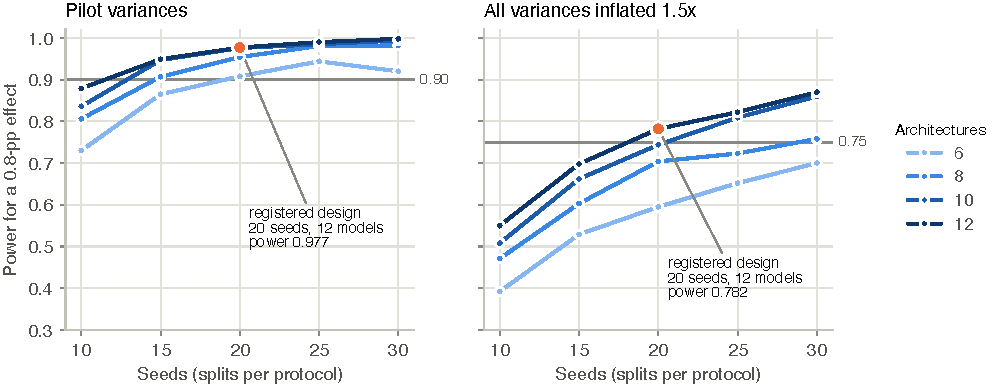
\includegraphics[width=\textwidth]{power.pdf}
\caption{Simulated power of the H1 model for a 0.8-pp effect (1,000 simulations per design).}
\label{r:fig:power}
\end{figure}

{\footnotesize
\setlength{\tabcolsep}{3.5pt}
\begin{longtable}{llrrrrr}
\caption{Simulated power (1,000 simulations per cell) of the registered H1 model for a 0.8-pp effect, by variance scale, number of architectures, and number of seeds.}\label{r:tab:power}\\
\toprule
Variance & Archs & 10 seeds & 15 seeds & 20 seeds & 25 seeds & 30 seeds \\
\midrule
\endfirsthead
\toprule
Variance & Archs & 10 seeds & 15 seeds & 20 seeds & 25 seeds & 30 seeds \\
\midrule
\endhead
\bottomrule
\endfoot
1$\times$ & 6 & 0.730 & 0.865 & 0.908 & 0.944 & 0.920 \\
1$\times$ & 8 & 0.806 & 0.907 & 0.954 & 0.981 & 0.982 \\
1$\times$ & 10 & 0.836 & 0.947 & 0.976 & 0.985 & 0.994 \\
1$\times$ & 12 & 0.879 & 0.949 & 0.977 & 0.990 & 0.998 \\
1.5$\times$ & 6 & 0.392 & 0.529 & 0.595 & 0.652 & 0.700 \\
1.5$\times$ & 8 & 0.471 & 0.603 & 0.704 & 0.723 & 0.758 \\
1.5$\times$ & 10 & 0.508 & 0.662 & 0.744 & 0.809 & 0.860 \\
1.5$\times$ & 12 & 0.550 & 0.698 & 0.782 & 0.822 & 0.870 \\
\end{longtable}
}


\chapter{The designs in detail}
\label{r:ch:designs}

\begin{figure}[H]
\centering
\begin{adjustbox}{max width=\textwidth}
\begin{tikzpicture}[node distance=3mm and 4mm]
\node[box=34mm] (p1) {\textbf{Phase 1} (H1)\\12 archs $\times$ 20 seeds $\times$ P1, P2, P3\\= 720 runs};
\node[box=34mm, right=of p1] (fc) {\textbf{2C / 2B} (H3, H4)\\4 archs $\times$ 10 seeds $\times$ 4 cells\\= 160 runs + composites};
\node[box=34mm, right=of fc] (gr) {\textbf{2A} (H5)\\2 archs $\times$ 10 seeds $\times$ 7 $\lambda$ $\times$ P1, P2\\= 280 runs};
\node[box=34mm, below=of fc] (cr) {\textbf{CRIC} (H2)\\6 archs $\times$ 10 seeds $\times$ P1, P1$'$, P2\\= 180 runs};
\node[box=34mm, left=of cr] (fp) {\textbf{Fingerprint encoder}\\1 run (secondary)};
\node[done=34mm, right=of cr] (tot) {\textbf{1,341 runs}\\one registration commit};
\end{tikzpicture}
\end{adjustbox}
\caption{The registered Study 2 run matrix. P1-prime equals P1 byte for byte on every SIPaKMeD seed (P2 always has
exactly 810 test crops), so it needed no separate SIPaKMeD runs.}
\label{r:fig:study2-matrix}
\end{figure}


\section{Splits}

P1 is a stratified 80:20 crop split; P2 a parent-disjoint split taken from \texttt{StratifiedGroupKFold} as the fold
whose test size is closest to 810 crops; P3 the same on near-duplicate component groups. For every SIPaKMeD seed P2 has
exactly 810 test crops, so P1-prime (a P1 split resampled to P2's size) is byte-identical to P1 and was not trained
separately. For CRIC, P1-prime differs from P1 by 2--11 training cells and was trained.

\section{Architectures}

{\footnotesize
\setlength{\tabcolsep}{3.5pt}
\begin{longtable}{llp{4.6cm}rr}
\caption{The twelve Study 2 backbones: penultimate feature dimension, ImageNet weights, and mean Phase 1 training and total minutes per run.}\label{r:tab:archs}\\
\toprule
Architecture & Dim & Weights & Train min & Total min \\
\midrule
\endfirsthead
\toprule
Architecture & Dim & Weights & Train min & Total min \\
\midrule
\endhead
\bottomrule
\endfoot
ResNet-18 & 512 & ResNet18\_\allowbreak{}Weights.\allowbreak{}IMAGENET1K\_\allowbreak{}V1 & 0.85 & 0.87 \\
ResNet-50 & 2048 & ResNet50\_\allowbreak{}Weights.\allowbreak{}IMAGENET1K\_\allowbreak{}V2 & 2.60 & 2.64 \\
DenseNet-121 & 1024 & DenseNet121\_\allowbreak{}Weights.\allowbreak{}IMAGENET1K\_\allowbreak{}V1 & 3.25 & 3.29 \\
EfficientNet-B0 & 1280 & EfficientNet\_\allowbreak{}B0\_\allowbreak{}Weights.\allowbreak{}IMAGENET1K\_\allowbreak{}V1 & 1.78 & 1.80 \\
MobileNet-V2 & 1280 & MobileNet\_\allowbreak{}V2\_\allowbreak{}Weights.\allowbreak{}IMAGENET1K\_\allowbreak{}V2 & 1.45 & 1.48 \\
ViT-B/16 & 768 & ViT\_\allowbreak{}B\_\allowbreak{}16\_\allowbreak{}Weights.\allowbreak{}IMAGENET1K\_\allowbreak{}V1 & 9.09 & 9.17 \\
ConvNeXt-T & 768 & ConvNeXt\_\allowbreak{}Tiny\_\allowbreak{}Weights.\allowbreak{}IMAGENET1K\_\allowbreak{}V1 & 5.15 & 5.21 \\
Swin-T & 768 & Swin\_\allowbreak{}T\_\allowbreak{}Weights.\allowbreak{}IMAGENET1K\_\allowbreak{}V1 & 4.61 & 4.66 \\
RegNetY-1.6GF & 888 & RegNet\_\allowbreak{}Y\_\allowbreak{}1\_\allowbreak{}6GF\_\allowbreak{}Weights.\allowbreak{}IMAGENET1K\_\allowbreak{}V2 & 2.47 & 2.50 \\
EfficientNetV2-S & 1280 & EfficientNet\_\allowbreak{}V2\_\allowbreak{}S\_\allowbreak{}Weights.\allowbreak{}IMAGENET1K\_\allowbreak{}V1 & 3.46 & 3.50 \\
MaxViT-T & 512 & MaxVit\_\allowbreak{}T\_\allowbreak{}Weights.\allowbreak{}IMAGENET1K\_\allowbreak{}V1 & 7.76 & 7.86 \\
DINOv2 ViT-S/14 & 384 & timm:vit\_\allowbreak{}small\_\allowbreak{}patch14\_\allowbreak{}dinov2.\allowbreak{}lvd142m & 4.08 & 4.13 \\
\end{longtable}
}


\section{2C: leakage at matched diversity}

\begin{figure}[H]
\centering
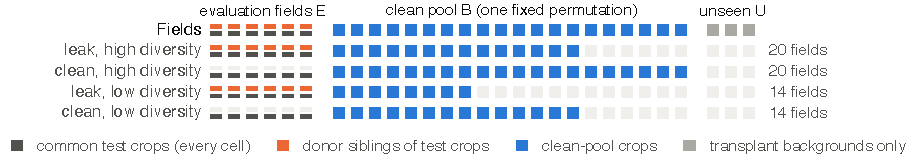
\includegraphics[width=\textwidth]{design.pdf}
\caption{The 2C factorial for one seed: one common test set; leak cells add the evaluation fields' sibling crops, clean
cells use other fields; within a diversity level crop and field counts are identical, and low-diversity field sets are
nested in high-diversity ones.}
\label{r:fig:design}
\end{figure}

For each seed and class, 30\% of fields with at least two crops are evaluation fields; half of each one's crops (rounded
down) form the common test set (about 527 crops) and the rest are its donor siblings. Six fields per class with at least
three crops are reserved as unseen background donors for 2B. Each training set holds exactly 220 crops per class. The
clean cells draw from non-evaluation fields along one fixed permutation; the leak cells replace the last $|E|$ fields of
that permutation with the evaluation fields' donor siblings; the low-diversity cells use the first 70\% of the
permutation. High-diversity cells therefore contain 720 distinct fields and low-diversity cells 504. Every test crop
has a training sibling in the leak cells (2.0 on average at high diversity, 3.0 at low) and none in the clean cells. A
240-crop budget was infeasible for seed 307 and for 10 of 100 unrelated seeds, so 220 was chosen before any training;
it was feasible for 100 of 100.

\section{2B: counterfactual background transplants}

\begin{figure}[H]
\centering
\begin{adjustbox}{max width=\textwidth}
\begin{tikzpicture}[node distance=3mm and 4mm]
\node[box=22mm] (orig) {Original test cell};
\node[box=22mm, right=of orig] (mask) {Foreground mask\\\footnotesize Otsu (S, Y) + close};
\node[box=22mm, right=of mask] (inp) {Donor background\\\footnotesize Telea inpainting};
\node[box=22mm, right=of inp] (comp) {Feathered composite\\\footnotesize $\sigma=2$ px};
\node[box=21mm, below=7mm of orig] (self) {\textbf{self}\\own background};
\node[box=21mm, right=of self] (sib) {\textbf{sibling}\\same field};
\node[box=21mm, right=of sib] (same) {\textbf{unseen same}\\unseen field, same class};
\node[box=21mm, right=of same] (other) {\textbf{unseen other}\\unseen fields, other classes};
\draw[flow] (orig) -- (mask); \draw[flow] (mask) -- (inp); \draw[flow] (inp) -- (comp);
\draw[decorate,decoration={brace,amplitude=4pt,mirror}] (self.south west) -- (other.south east)
  node[midway, below=5pt, note] {route = acc(sibling) $-$ acc(unseen same); H4 = leak $-$ clean difference of the route};
\end{tikzpicture}
\end{adjustbox}
\caption{The 2B counterfactual background transplants. The \emph{self} condition measures seam and inpainting artifacts;
every contrast compares conditions that share them.}
\label{r:fig:transplant-diagram}
\end{figure}


\section{2A: adversarial fingerprint suppression}

\begin{figure}[H]
\centering
\begin{adjustbox}{max width=\textwidth}
\begin{tikzpicture}[node distance=4mm and 6mm]
\node[box=22mm] (x) {Augmented crop};
\node[box=24mm, right=of x] (bb) {Backbone\\\footnotesize ImageNet init};
\node[box=22mm, right=of bb] (f) {Pooled features $z$};
\node[box=24mm, above right=2mm and 6mm of f] (head) {Class head\\\footnotesize linear};
\node[gold=24mm, below right=2mm and 6mm of f] (grl) {Gradient reversal\\\footnotesize $\times(-\lambda_t)$, DANN ramp};
\node[box=28mm, right=of grl] (adv) {Parent head\\\footnotesize 2A: MLP 512\\\footnotesize A8: BN + linear, reset /5 ep};
\node[box=26mm, right=of adv] (mask) {Mask to parents of the true class};
\node[box=20mm, right=of head] (ce) {Class CE};
\draw[flow] (x) -- (bb); \draw[flow] (bb) -- (f); \draw[flow] (f) |- (head); \draw[flow] (f) |- (grl);
\draw[flow] (grl) -- (adv); \draw[flow] (adv) -- (mask); \draw[flow] (head) -- (ce);
\end{tikzpicture}
\end{adjustbox}
\caption{The adversarial suppression arms. The parent adversary only competes among parents of the sample's own class,
so suppressing it never requires removing class information. Study 2 (2A) used a two-layer MLP; Amendment 8 (F7) used a
probe-matched head (per-feature standardisation and one linear layer, its own optimiser at $10^{-3}$, re-initialised every
five epochs) so that features could not hide parent identity from it while leaving it readable by a linear probe.}
\label{r:fig:adversary}
\end{figure}


The maximum reversal coefficient followed the DANN ramp $\lambda\,(2/(1+e^{-10p})-1)$ over training progress $p$, with
$\lambda\in\{0, 0.01, 0.03, 0.1, 0.3, 1, 3\}$. Recoverability $R$ is the within-class field-identification accuracy of a
multinomial logistic regression (C = 1, standardised features) on frozen features of the balanced 424-field probe split
(two fitting and two evaluation crops per field). The \emph{regime} is the set of $\lambda$ whose mean P2 accuracy stays
within 1~pp of $\lambda=0$; the \emph{manipulation check} requires $R$ at the strongest in-regime $\lambda$ to fall by at
least a quarter of its above-floor baseline.

\section{CRIC}

CRIC cells are $100\times100$ windows centred on the published nucleus coordinates (shifted inward at image borders) of
the 400 Figshare slide images, whose MD5 and SHA-256 were verified (\artifact{data_manifests/cric_images_verified.json}).
Six Bethesda classes; ResNet-18, ResNet-50, DenseNet-121, EfficientNet-B0, ConvNeXt-T, ViT-B/16; P1, P1-prime, P2; ten
seeds.

\chapter{Structure before training}
\label{r:ch:structure}

For a parent with $k$ crops allocated independently with test fraction $q$, the parent straddles the split with
probability $1-(1-q)^k-q^k$; a test crop has a training sibling with probability $1-q^{k-1}$ and $(1-q)(k-1)$ training
siblings on average; and the ratio of distinct training parents between a crop-level and a parent-level split of equal
size is $\sum_j\{1-q^{k_j}\}/\{(1-q)m\}$ for $m$ parents. Class--parent dependence is the mutual information between
parent and class divided by the class entropy. \texttt{cytofair risk-report} computes all of them from any crop-to-parent
table (\artifact{src/cytofair/risk.py}).

{\scriptsize
\setlength{\tabcolsep}{3.5pt}
\begin{longtable}{lrrrrrrrr}
\caption{\texttt{cytofair risk-report} closed forms for the four datasets at a 20\% test fraction: crops per parent, expected straddle and sibling rates (percent), siblings per test crop, training-diversity ratio, and class--parent dependence (fraction of class entropy explained by the parent).}\label{r:tab:risk}\\
\toprule
Dataset & Obs. & Parents & Obs./parent & Straddle & Test w/ sibling & Siblings & Diversity & Class dep. \\
\midrule
\endfirsthead
\toprule
Dataset & Obs. & Parents & Obs./parent & Straddle & Test w/ sibling & Siblings & Diversity & Class dep. \\
\midrule
\endhead
\bottomrule
\endfoot
SIPaKMeD & 4,049 & 966 & 4.19 & 44.8 & 91.7 & 5.16 & 1.176 & 1.000 \\
Cx22 & 1,320 & 514 & 2.57 & 33.9 & 83.6 & 1.95 & 1.164 & -- \\
CRIC & 11,534 & 400 & 28.84 & 94.9 & 100.0 & 35.56 & 1.250 & 0.676 \\
Herlev & 917 & 917 & 1.00 & 0.0 & 0.0 & 0.00 & 1.000 & 1.000 \\
\end{longtable}
}


\begin{figure}[H]
\centering
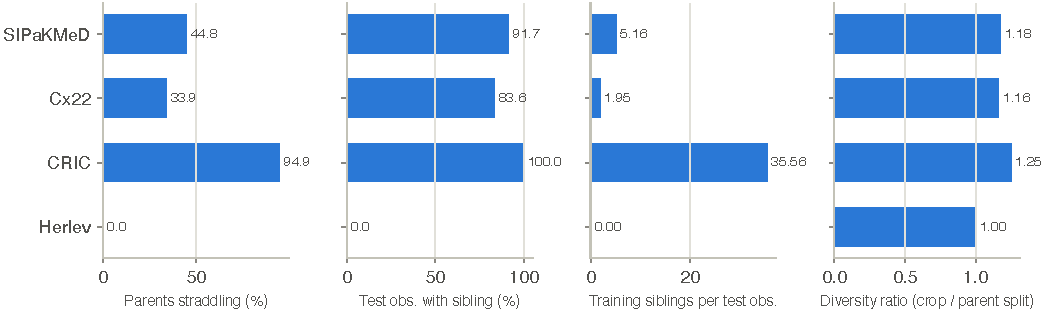
\includegraphics[width=\textwidth]{structure.pdf}
\caption{Closed-form structural exposure of the four datasets to a random 80:20 crop split.}
\label{r:fig:structure}
\end{figure}

Under five random P1 splits, the share of test observations sharing at least one source pixel with a training
observation was \RecOverlapSip\% for SIPaKMeD, \RecOverlapCric\% for CRIC, and \RecOverlapCx\% for Cx22
(\artifact{results/study2/structural/literal_overlap_p1.csv}). CRIC is exposed on every measure: 29 cells per slide image,
essentially every test cell with a training sibling, and slide identity explaining two thirds of the class entropy.
That is the structure that predicted, before training, that CRIC's inflation would be the largest.
